\documentclass{article}

\textwidth=6.5in
\textheight=8.5in
\voffset=-54pt
\oddsidemargin=0in
\evensidemargin=0in
\setlength{\parskip}{8pt}
\setlength{\parindent}{0pt}

\usepackage{workbook}

\usepackage[]{handout}

\begin{document}

\begin{center}
  \large\textsc{Problem Set 15 - Derivatives of Inverse Trigonometric Functions}
  
      \pspace{12pt}
  \begin{problemonly}\large Name: \rule{5cm}{0.15mm}\\ \end{problemonly}
\end{center}

\begin{grading}
\begin{enumerate}
    \item 15 points, 3 for each part.
    \item 10 points, as follows: 2/3/2/3
    \item 10 points, as follows: 2/2/3/3
    \item 10 points, as follows: 2/1/1/2/1/1
    \item 20 points, as follows: 2/2/4/3/3/2/4
    \item 13 points, 1 for reach row in the table
\end{enumerate}
Total: 78 points.
\end{grading}

\begin{enumerate}

\item 

\begin{grading}
    15 points. 3 for each part. 
\end{grading}

  Simplify each of the following to an expression that does not
  involve trigonometric functions or inverse trigonometric functions.

  \begin{enumerate}
  \item
    \begin{problem}[\vfill]
      $\sin\!\left(\cos^{-1}\!\left( - \frac{2}{3}\right)\right)$
    \end{problem}

    \begin{solution}
      We can use the same strategy as in {{\#4}} from the worksheet:
      $\cos^{-1}\left( - \frac{2}{3}\right)$ is the red angle below:
      \begin{center}
        \begin{tikzangle}[angle=rad(acos(-2/3)), func=cos,
          functick=$-\frac{2}{3}$, triangle=true]            
        \end{tikzangle}
      \end{center}
      The reference triangle has width $\frac{2}{3}$ and hypotenuse 1, so
      its height is $\frac{\sqrt{5}}{3}$ by the Pythagorean Theorem.
      Therefore, $\displaystyle
      \sin\left(\cos^{-1}\left(-\frac{2}{3}\right)\right) =
      \boxed{\frac{\sqrt{5}}{3}}$.

      \emph{Alternate method:} Instead of drawing the reference triangle,
      some people prefer drawing a triangle which is similar to the
      reference triangle but whose known side lengths are integers; for
      example, since the reference angle here has a cosine of
      $\frac{2}{3}$, we could draw a triangle like this (we've labeled the
      reference angle $\theta$):
      \begin{center}
        \begin{tikzangle}[angle=rad(acos(-2/3)), label=$\cos^{-1} \left( -
            \frac{2}{3} \right)$, labelpos=0.15]
          \pgfmathsetmacro{\y}{sqrt(5)} %
          \draw[blue, thick] (axis cs: 0, 0) -- node[below] {length 2}
          (axis cs: -2, 0) -- (axis cs: -2, \y) -- (axis cs: 0, 0); %
          \draw[blue, decorate, decoration={text along path, text={length
              3}, text align={center}, text color={blue}, raise=4pt}]
          (axis cs: -2, \y) -- (axis cs: 0, 0); %
          \draw[blue] ($(axis cs: 0, 0) - (8pt, 0)$) arc[radius=8pt,
          start angle=180, end angle=acos(-2/3)]; %
          \draw[blue] ($(axis cs: 0, 0) + (-12pt, 4pt)$) node{$\theta$};
        \end{tikzangle}
      \end{center}
      By the Pythagorean Theorem, the blue triangle has height $\sqrt{5}$,
      so $\sin \theta = \frac{\sqrt{5}}{3}$.  Therefore, $\sin \left(
        \cos^{-1} \left( - \frac{2}{3} \right) \right)$ is also equal to
      $\frac{\sqrt{5}}{3}$.  (Note that the unit circle itself isn't
      important in this picture, and we could leave it out.)
    \end{solution}

  \item
    \begin{problem}[\vfill]
      $\sin\!\left(\arctan (-2) \right)$
    \end{problem}      

    \begin{solution}
      $\arctan (-2)$ is the angle in $\left( - \frac{\pi}{2},
        \frac{\pi}{2} \right)$ whose tangent value is $-2$.  In
      particular, since its tangent value is negative, it must lie in
      $\left( - \frac{\pi}{2}, 0 \right)$.  We can picture $\arctan (-2)$
      like this:
      \begin{center}
        \begin{tikzangle}[angle=rad(atan(-2))]
          \draw[red] (axis cs: \px, \py) node[anchor=north west]{slope
            $-2$};
        \end{tikzangle}
      \end{center}
      If we extend this terminal side further, we could, for example, make
      a triangle with width 1 and height 2 (so that the slope of the
      hypotenuse is $-2$):
      \begin{center}
        \begin{tikzangle}[angle=rad(atan(-2))]
          \draw[blue, thick] (axis cs: 0, 0) -- (axis cs: 1, -2) --
          node[right] {2} (axis cs:
          1, 0) -- node[above] {1} (axis cs: 0, 0);
        \end{tikzangle}
      \end{center}
      By the Pythagorean Theorem, this triangle has hypotenuse $\sqrt{5}$,
      so the sine value of the angle $\arctan(-2)$ is $\boxed{-
        \frac{2}{\sqrt{5}}}$.
    \end{solution}

  \item
    \begin{problem}[\vfill]
      $\arctan\! \left ( \tan 3 \pi \right )$
    \end{problem}

    \begin{solution}
      $\tan 3\pi = 0$, so this is asking for $\arctan 0$, which is
      $\boxed{0}$. 
    \end{solution}

  \item
    \begin{problem}[\vfill]
      $\sin(\arccos x)$, where $x\geq0$.
    \end{problem}

    \begin{solution}
      $\arccos x$ is the angle in $[0,\pi]$ whose cosine is $x$.
      Since $x \geq 0$, $\arccos x$ is in $[0,\frac{\pi}{2}]$. The sine of
      any angle in this interval is non-negative.
      The relevant reference triangle looks like this:
      \begin{center}
        \begin{tikzpicture}[scale=0.7]
            \coordinate (O) at (0,0);
            \coordinate (A) at (3,0);
            \coordinate (B) at (3,4);
            \draw (O) -- (A) -- (B) -- cycle;
            \draw (2.4,0.6) rectangle (3,0);
            \draw pic[draw=black,angle radius=15,
            "$\theta$"] {angle=A--O--B};
            \path (O) -- node[below] {$|x|$} (A) --
            node[right] {$\sqrt{1-|x|^2}$} (B) -- node[above left=-2pt]
            {$1$} cycle;
        \end{tikzpicture}
      \end{center}
       By the Pythagorean Theorem, this opposite side has length $\sqrt{1 -
        |x|^2} = \sqrt{1 - x^2}$. The sign of $x$ does not affect the value, so 
      $\boxed{\sin(\arccos x)=\sqrt{1 - x^2}}$. 
    \end{solution}

  \item
    \begin{problem}[\vfill\newpage]
      $\sin(\arccos x)$, where $x<0$.
    \end{problem}

      \begin{solution}
      As in part (d), $\arccos x$ is the angle in $[0,\pi]$ whose cosine is $x$.
      Since $x < 0$, $\arccos x$ must be in $(\frac{\pi}{2},\pi]$. The sine
      of any angle in this interval is non-negative.
      
      By identical reasoning as in part (d),
      $\boxed{\sin(\arccos x)=\sqrt{1 - x^2}}$. 
    \end{solution}

  \end{enumerate}


\item 

\begin{grading}
    10 points, as follows: 2/3/2/3 
\end{grading}

If you'd like to review the technique
  we used to find the derivatives of $\arctan x$ and $\arcsin x$, read
  pages 703 - 705 in Gottlieb or the solutions to workbook section 3.5. Then do the following.

  Let $f(x) = \arccos x$.
  \begin{enumerate}
  \item
\begin{problem}[\stretch{2}]
      Sketch the graph of $f(x)$.  (Be sure to clearly indicate the domain
      and range!)
    \end{problem}

    \begin{solution}
      Here's the graph of $\arccos x$.  (See {{{Problem Set 10}, {{\#1}}}} for
        details.)
      \begin{center}
        \begin{tikzpicture}
          \begin{axis}[xtick={-1, 1}, ytick={-4.71239, -3.14159, -1.5708, 0.,
              1.5708, 3.14159, 4.71239}, yticklabels={$-\frac{3 \pi }{2}$,
              $-\pi$, $-\frac{\pi }{2}$, $0.$, $\frac{\pi }{2}$, $\pi$,
              $\frac{3 \pi }{2}$}, xmin=-1.75, xmax=1.75, ymin=0,
            ymax=3.5, clip=false, cycle list=black, width=2in, height=2in]
            \addplot[domain=-1:1] {rad(acos(x))};
            \addplot[only marks, mark=*, mark size=1.5pt] coordinates
            {
              (-1, 3.14159)
              (1, 0)
            };
          \end{axis}
        \end{tikzpicture}
      \end{center}      
    \end{solution}

  \item
    \begin{problem}[\stretch{2}]
      Find the derivative of $\arccos x$ using implicit differentiation.  
    \end{problem}

    \begin{solution}
      Let's write
      \begin{align*}
        y &= \arccos x \\
        \intertext{We'd like to find $\frac{dy}{dx}$, and we'll first
          rewrite this in terms of $\cos$ since we know how to
          differentiate $\cos$:}
        \cos y &= x \\
      \shortintertext{Differentiate both sides with respect to $x$:}
      \frac{d}{dx} (\cos y) &= \frac{d}{dx} (x) \\
      - \sin y \frac{dy}{dx} &= 1 \\
      \frac{dy}{dx} &= - \frac{1}{\sin y}
    \end{align*}
    As in {{\#1}} and
      {{\#2}} on the worksheet, we'd like to express this in terms of
      $x$.  The equation $y = \arccos x$ says that $y$ is the angle in
    $[0, \pi]$ whose cosine is $x$, and we can picture this statement
    graphically:
    \begin{center}
      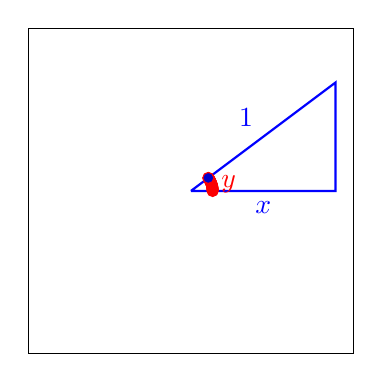
\begin{tikzpicture}
        \begin{axis}[axis equal=true, xmin=-4.5, xmax=4.5, ymin=-4.5,
          ymax=4.5, xtick=\empty, ytick=\empty, width=2.25in,
          height=2.25in, clip=false] %
          \draw[blue, thick] (axis cs: 0, 0) -- node[anchor=south east]
          {$1$} (axis cs: 4, 3) -- (axis cs: 4, 0) -- node[below]{$x$}
          (axis cs: 0, 0); %
          \pgfmathsetmacro{\angle}{atan(3/4)} %
          \addplot+[domain=0:\angle, red, thin, ->, >=to] ({0.6 * cos(x)},
          {0.6 * sin(x)}) node[pos=0.5, right] {$y$};
        \end{axis}
      \end{tikzpicture}        
    \end{center}
    By the Pythagorean Theorem, this triangle has height $\sqrt{1 - x^2}$,
    so $\sin y = \frac{\sqrt{1 - x^2}}{1} = \sqrt{1 - x^2}$.  Therefore,
    $\displaystyle \frac{dy}{dx} = - \frac{1}{\sin y} = \boxed{ -
      \frac{1}{\sqrt{1 - x^2}}}$. 
  \end{solution}    

  \item
    \begin{problem}[\vfill]
      Use your formula for $f'(x)$ to explain why $f$ is always decreasing
      (on its domain).
    \end{problem}

    \begin{solution}
      The expression $- \frac{1}{\sqrt{1 - x^2}}$ is always negative
      (where it's defined).
    \end{solution}

  \item
    \begin{problem}[\nstretch{2}]
      Find $f''(x)$, and use it to determine the intervals on which $f(x)
      = \arccos x$ is concave up and the intervals on which $f(x)$ is
      concave down.  Is this accurately reflected in the graph you
      sketched in {{{{\#2}}(a)}}? If not, go back and adjust your graph.
    \end{problem}

    \begin{solution}
      We can write $f'(x) = - (1 - x^2)^{-1/2}$, so $\displaystyle f''(x)
      = \frac{1}{2} (1 - x^2)^{-3/2} (-2x) = \boxed{ - \frac{x}{(1 -
          x^2)^{3/2}}}$.  To determine when $f$ is concave up and when
      it's concave down, we'll make a sign chart for $f''$.  First, $f''$
      is undefined when its denominator is 0, which happens when $x = \pm
      1$; it is 0 when its numerator is 0, which happens when $x = 0$.  By
      testing points, we get the following sign chart for $f''$:
      \begin{center}
        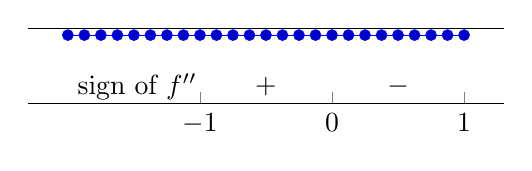
\begin{tikzpicture}
          \begin{axis}[axis y line=none, x axis line style={-}, xtick={-1., 0., 1.}, xticklabels={$-1$, $0$, $1$}, ymin=-2, height=1in, width=3in]
            \addplot+[domain=-2.:1., very thin]{0};
            \draw (axis cs: -2., -1.5) node[right] {sign of $f''$};
            \draw (axis cs: -0.5, -1.5) node{$+$};
            \draw (axis cs: 0.5, -1.5) node{$-$};
          \end{axis}
        \end{tikzpicture}
      \end{center}
      So, \fbox{$f$ is concave up on $(-1, 0)$ and concave down on $(0,
        1)$}, which agrees with our sketch of $f$.  It also agrees with
      our sketch of $f'$ because it says that $f'$ is increasing on $(-1,
      0)$ and decreasing on $(0, 1)$.
    \end{solution}

  \end{enumerate}

\item 

\begin{grading}
    10 points, as follows: 2/2/3/3
\end{grading}

 Find the derivatives of the following functions. For help,
  look at Example 21.4 on page 705 in Gottlieb.

    \begin{enumerate}
    \item
      \begin{problem}[\vfill]
        $(\arcsin x)^2$ $\vphantom{\dfrac{1}{1}}$
      \end{problem}

      \begin{solution}
        $\displaystyle \frac{d}{dx}
        \left(\fcolorbox{red}{white}{$\displaystyle
            \fcolorbox{blue}{white}{$\displaystyle \left( \arcsin {x} 
              \right)$}^ { 2} $}\right) = \boxed{2 \left( \arcsin{x} x
          \right) \cdot \frac{1}{\sqrt{1-x^2}}}$.
      \end{solution}

    \item
      \begin{problem}[\vfill]
        $\arcsin (x^2)$ $\vphantom{\dfrac{1}{1}}$
      \end{problem}

      \begin{solution}
        $\displaystyle \frac{d}{dx}
        \left(\fcolorbox{red}{white}{$\displaystyle \arcsin\left(\fcolorbox{blue}{white}{$\displaystyle x^ { 2}
                $}\right)$}\right) = \boxed{\frac{1}{\sqrt{1-\left(x^ { 2}
              \right)^2}}\cdot \left(2 x\right)}$.
      \end{solution}

    \item
      \begin{problem}[\vfill]
        $(\arccos x)(\ln x)$ $\vphantom{\dfrac{1}{1}}$
      \end{problem}

      \begin{solution}
        Here, we need the Product Rule: $\displaystyle \frac{d}{dx}
        \left(\fcolorbox{green}{white}{$\displaystyle \arccos x$}\cdot
          \fcolorbox{green}{white}{$\displaystyle \ln x$}\right) =
        \boxed{\arccos x\cdot \frac{1}{x}-\frac{1}{\sqrt{1-x^2}}\cdot \ln
          x}$.
      \end{solution}

    \item
      \begin{problem}[\vfill\newpage]
        $\dfrac{(\tan x)(\arctan x)}{\pi}$
      \end{problem}

      \begin{solution}
        First, we can think of the given function as $\frac{1}{\pi} (\tan
        x)(\arctan x)$, and $\frac{1}{\pi}$ is just a constant multiple;
        then, we use the Product Rule to get that the derivative is 
        $\boxed{\frac{\arctan x \cdot \sec^2 x +
            \frac{1}{x^2+1}\cdot \tan x}{\pi}}$.
      \end{solution}

    \end{enumerate}

\item 

\begin{grading}
    10 points, as follows: 2/1/1/2/1/1
\end{grading}

Let $f(x) = \arcsin x + \arccos x$.
  \begin{enumerate}
  \item
\begin{problem}[\vfill]
      Find $f'(x)$.
    \end{problem}

    \begin{solution}
      The derivative of $\arcsin x$ is $\frac{1}{\sqrt{1 - x^2}}$, and the
      derivative of $\arccos x$ is $-\frac{1}{\sqrt{1 - x^2}}$, so $f'(x)
      = \frac{1}{\sqrt{1 - x^2}} - \frac{1}{\sqrt{1 - x^2}} = \boxed{0}$. 
    \end{solution}

  \item
    \begin{problem}[\vfill]
      What does your answer to {{{{\#4}}(a)}} tell
      you about the graph of $f(x)$?
    \end{problem}

    \begin{solution}
      The fact that the derivative is 0 everywhere says that $f(x)$ must
      be a constant function.
    \end{solution}

  \item
    \begin{problem}[\vfill]
      What is the domain of $f(x)$?
    \end{problem}

    \begin{solution}
      $\arcsin x$ and $\arccos x$ both have domain $[-1, 1]$, so the
      domain of $f(x)$ is also $[-1, 1]$. 
    \end{solution}

  \item
    \begin{problem}[\stretch{2}]
      Sketch the graph of $f(x)$.
    \end{problem}

    \begin{solution}
      We know that $f(x)$ is a constant function with domain $[-1, 1]$.
      This tells us that the graph should just be a horizontal line
      segment from $x = -1$ to $x = 1$.  What we need to know is the
      vertical position of this line.  To do this, let's figure out one
      value of $f$, like $f(0)$.

      By definition, $f(0) = \arcsin 0 + \arccos 0 = 0 + \frac{\pi}{2} =
      \frac{\pi}{2}$.  So, $f(x)$ is the constant function $\frac{\pi}{2}$
      with domain $[-1, 1]$:
      \begin{center}
        \begin{tikzpicture}
          \begin{axis}[xtick={-1, 1}, ytick={1.57},
            yticklabels={$\frac{\pi}{2}$}, ymin=0, cycle list=black,
            width=2in, xmin=-1.5, xmax=1.5]
            \addplot+[domain=-1:1] {pi/2};
            \addplot+[only marks, mark=*, mark size=1.5pt] coordinates
            {
              (-1, 1.57)
              (1, 1.57)
            };
          \end{axis}
        \end{tikzpicture}
      \end{center}
    \end{solution}

  \item
    \begin{problem}[\vfill]
      Based on your graph, write a simpler formula for $f(x)$.  
    \end{problem}

    \begin{solution}
      As we've seen already, $f(x) = \boxed{\frac{\pi}{2}}$.  
    \end{solution}

  \item
    \begin{problem}[\nstretch{2}]
      Use a right triangle to explain why your formula is reasonable when
      $x$ is positive.
    \end{problem}

    \begin{solution}
      If $x$ is positive, we'd like to explain why $\arcsin x + \arccos x
      = \frac{\pi}{2}$.  We can see this by drawing a right triangle with
      one leg of length $x$ and hypotenuse of length $1$:
      \begin{center}
        \begin{tikzpicture}[x=1.5cm, y=1.5cm]
          \coordinate (A) at (0,0);
          \coordinate (B) at (1, 2);
          \coordinate (C) at (1,0);
          \draw (0, 0) -- node[anchor=south east]{$1$} (B) -- (B |- 0, 0)
          -- node[below] {$x$} (0, 0); %
          \draw ($(B |- 0, 0) - (8pt, 0)$) -- ++(0, 8pt) -- ++(8pt, 0); %
          \draw pic[draw=red, angle radius=8,
          "\textcolor{red}{$A$}",
          angle eccentricity = 1.8] {angle=C--A--B};
          \draw pic[draw=blue, angle radius=10,
          "\textcolor{blue}{$B$}",
          angle eccentricity = 1.8] {angle=A--B--C};
        \end{tikzpicture}
      \end{center}
      Notice that $\cos A = x$; since $A$ is an acute angle, $A = \arccos
      x$.  Similarly, $\sin B = x$; since $B$ is an acute angle, $B =
      \arcsin x$.  So, $\arccos x + \arcsin x = A + B = 90^\circ =
      \frac{\pi}{2}$.
    \end{solution}

  \end{enumerate}

\item 

\begin{grading}
    20 points, as follows: 2/2/4/3/3/2/4
\end{grading}

In this problem, you'll look at $f(x) = \arctan( \frac{1}{x})$.
  \begin{enumerate}

  \item
    \begin{problem}[\vfill]
      What is the domain of $f(x)$?
    \end{problem}

    \begin{solution}
      $\arctan \left( \frac{1}{x} \right)$ is defined as long as
      $\frac{1}{x}$ is, which happens for \fbox{all $x \neq 0$}. 
    \end{solution}

  \item
    \begin{problem}[\vfill]
      Is $f$ an even function, an odd function, or neither?
    \end{problem}

    \begin{solution} 
      To decide this, we look at $f(-x)$:
      \begin{align*}
        f(-x) &= \arctan \left( \frac{1}{-x} \right) \\
        \intertext{Since $\arctan$ is an odd function (which we can see
          from its graph), $\arctan(-u) = - \arctan (u)$; applying this to
          $u = \frac{1}{x}$, we can rewrite the previous line as}
        &= - \arctan \left( \frac{1}{x} \right) \\
        &= - f(x),
      \end{align*}
      so $f(x)$ is \fbox{odd}. 
    \end{solution}

  \item
    \begin{problem}[\stretch{2}]
      $f(x)$ is undefined at $x = 0$; calculate $\displaystyle \lim_{x \to
        0^+} f(x)$ and $\displaystyle \lim_{x \to 0^-} f(x)$. 
    \end{problem}

    \begin{solution}
      As $x \to 0^+$, $\frac{1}{x} \to \infty$, so $\boxed{ \lim_{x \to
          0^+} \arctan \left( \frac{1}{x} \right) = \frac{\pi}{2}}$.
      (When $x$ is a tiny positive number, evaluating $\arctan \left(
        \frac{1}{x} \right)$ involves taking $\arctan$ of a huge positive
      number, which gives an answer close to $\frac{\pi}{2}$.)

      As $x \to 0^-$, $\frac{1}{x} \to -\infty$, so $\boxed{\lim_{x \to
          0^-} \arctan \left( \frac{1}{x} \right) = - \frac{\pi}{2}}$.
      (Alternatively, we can simply use the fact that $f$ is odd to say
      that $\displaystyle \lim_{x \to 0^-} f(x)$ must be the negative of
      $\displaystyle \lim_{x \to 0^+} f(x)$.)
    \end{solution}

  \item
    \begin{problem}[\nstretch{3}]
      On what intervals is $f(x)$ increasing?  On what intervals is $f(x)$
      decreasing?  
    \end{problem}

    \begin{solution}
      Let's make a sign chart for $f'$.  First, we differentiate $f$,
      using the Chain Rule:
      \begin{align*}
        f'(x) &= \frac{1}{1 + \left( \frac{1}{x} \right)^2} \cdot \left( -
          x^{-2} \right) \\
        \intertext{Note that this is undefined when $x = 0$ (which we knew
          already because $f$ is undefined at $x = 0$); as long as $x \neq
          0$, we can simplify this to}
        &= \left( \frac{1}{1 + \frac{1}{x^2}}  \right) \left( -
          \frac{1}{x^2} \right) \\
        &= - \frac{1}{\left( 1 + \frac{1}{x^2} \right) x^2} \\
        &= - \frac{1}{x^2 + 1}
      \end{align*}      
      This is always negative, so \fbox{$f$ is decreasing on $(-\infty,
        0)$ and on $(0, \infty)$}.  (Since $f$ is undefined at $x = 0$, we
      don't say that $f$ is decreasing on all of $(-\infty,
      \infty)$.)
      \begin{center}
        \begin{tikzpicture}
          \begin{axis}[axis y line=none, x axis line style={-}, xtick={0},
          xticklabels={$0$}, ymin=-2, ymax=3, height=1.5in, width=3in,
          clip=false]
            \addplot+[domain=-4:2, very thin]{0};
            \draw (-4,0) node[above right] {$f$};
            \draw (-4,0) node[below right] {sign of $f'$};
            \draw (-1,0) node[below] {$-$};
            \draw (1,0) node[below] {$-$};
            \draw[black] (-2,1.5) -- (0,0.5);
            \draw[black] (0,2.5) -- (2,1.5);
            \addplot[open] coordinates {(0,0.5) (0,2.5)};
          \end{axis}
        \end{tikzpicture}
      \end{center}
    \end{solution}

  \item
    \begin{problem}[\vfill]
      On what intervals is $f(x)$ concave up? 
    \end{problem}

    \begin{solution}
      We'd like to make a sign chart for $f''$.  First, let's rewrite
      $f'(x) = - (x^2 + 1)^{-1}$ to make it easier to differentiate.  By
      the Chain Rule, $\displaystyle f''(x) = (x^2 + 1)^{-2} \cdot 2x =
      \frac{2x}{(x^2 + 1)^2}$.  Remember that $f$ is undefined at $0$, so
      $f''$ is also undefined at $0$; other than that, $f''$ is never
      undefined or 0.  So, the only interesting point in our sign chart is
      at $x = 0$.  We can test values to get the following sign chart for
      $f''$:
        \begin{center}
        \begin{tikzpicture}
          \begin{axis}[axis y line=none, x axis line style={-}, xtick={0},
          xticklabels={$0$}, ymin=-2, ymax=4, height=2in, width=3in,
          clip=false]
          
            \addplot+[domain=-4:2,black]{1};
            \draw (-4,1) node[above right] {$f$};
            \draw (-4,1) node[below right] {sign of $f'$};
            \draw[black,line width=0.1pt] (0,1.1) -- (0,0.9);
            \draw (0,1) node[below] {$0$};
            \draw (-1,1) node[below] {$-$};
            \draw (1,1) node[below] {$-$};
            \addplot[black,domain=-2:-0.05]{0.5*rad(atan(1/x))+2};
            \addplot[black,domain=0.05:2]{0.5*rad(atan(1/x))+2};
            \addplot[open] coordinates {(0,-pi/4+2) (0,pi/4+2)};

            \addplot[domain=-4:2,black]{0};
            \draw (-4,0) node[below right] {sign of $f''$};
            \draw (-1,0) node[below] {$-$};
            \draw (1,0) node[below] {$+$};
          \end{axis}
        \end{tikzpicture}
      \end{center}
      So, $f$ is concave up on $(0, \infty)$. 
    \end{solution}

  \item
    \begin{problem}[\vfill]
      Find all horizontal asymptotes of $f$ by evaluating $\displaystyle
      \lim_{x \to \infty} f(x)$ and $\displaystyle \lim_{x \to -\infty} f(x)$.
    \end{problem}

    \begin{solution}
      As $x \to \infty$, $\frac{1}{x} \to 0$, so $\boxed{\lim_{x \to
          \infty} \arctan \left( \frac{1}{x} \right) = 0}$ (if this is
      confusing, imagine plugging a huge positive number in for $x$:
      $\arctan \left( \frac{1}{x} \right)$ will involve taking $\arctan$
      of a tiny positive number, which gives a result close to 0).

      We can reason the same way about $\displaystyle \lim_{x \to -\infty}
      f(x)$, or we can use the fact that $f$ is odd to conclude that
      $\boxed{\displaystyle \lim_{x \to -\infty} f(x) = - \lim_{x \to
          \infty} f(x) = 0}$ as well.

      So, there is \fbox{one horizontal asymptote, $y = 0$}. 
    \end{solution}

  \item
    \begin{problem}[\stretch{2}]
      Sketch the graph of $f$; your graph should incorporate all of the
      information above. 
    \end{problem}

    \begin{solution} % Jason Bland
      \begin{center}
        \begin{tikzpicture}
          \begin{axis}[xmin=-5, xmax=5, xtick=\empty, ytick={-1.571, 0,
              1.571}, yticklabels={$-\frac{\pi}{2}$, 0, $\frac{\pi}{2}$},
            cycle list=black]
            \addplot+[domain=-5:-0.01] {(pi / 180) * atan(1 / x)};
            \addplot+[domain=0.01:5] {(pi / 180) * atan(1 / x)};
            \addplot[only marks, mark=*, fill=white] coordinates
            {
              (0, 1.571)
              (0, -1.571)
            };
          \end{axis}
        \end{tikzpicture}
      \end{center}
      \checkmark\ 
        Here are the key features the graph should have (based on the
        previous parts):
        \begin{itemize}[nosep]
        \item It's defined everywhere except at $x = 0$.
        \item $\displaystyle \lim_{x \to 0^+} f(x) = \frac{\pi}{2}$ and
          $\displaystyle \lim_{x \to \infty} f(x) = 0$.
        \item It is decreasing and concave up on $(0, \infty)$.
        \item It's symmetric about the origin (because $f$ is odd).
        \end{itemize}
    \end{solution}

  \end{enumerate}

  \probonly{\emph{You are encouraged to check your work by graphing $f(x)$
      with a calculator or computer.}}

\spaceonly{\pspace{\newpage}}

\item 

\begin{grading}
    13 points, 1 for each row in the table.
\end{grading}

 \textbf{Reflect Back.}

  It may be surprising to you that the derivatives of inverse trig
  functions do not involve trig at all. Fill in the following table, being
  sure to use inverse trig functions as appropriate. (You'll use them
  twice below.)  When you're filling in the left column, there will be
  infinitely many functions (for instance, $x^2$ and $x^2 + 1$ both have
  derivative $2x$); just write one of them.  (Don't forget about the Chain
  Rule!)

  Note: Inverse trig derivatives figure prominently when we think about
  ``undoing" differentiation, hence the value of this exercise.
\vspace{-12pt}
  \begin{center}
    \renewcommand{\arraystretch}{2.4}
    \begin{tabular}{c|c}
      $f(x)$ & $f'(x)$ \\
      \hline
     $\dfrac{x^5}{5}$ & \solonly{$x^4$} \probonly{\hspace{1in}} \\
      \hline
      \probonly{\hspace{1in}}\solonly{ $\dfrac{x^4}{4}$} & $x^3$ \\
      \hline
      $e^{3x}$ & \solonly{$3e^{3x}$} \\
      \hline
      \solonly{ $\dfrac{1}{3}e^{3x}$}& $e^{3x}$ \\
      \hline
      $\ln x$ & \solonly{$\dfrac{1}{x}$} \\
      \hline
      \solonly{$\ln(x+1)$} & $\dfrac{1}{x + 1}$ \\
      \hline
      $\ln (3x + 1)$ & \solonly{$\dfrac{3}{3x+1}$}\\
      \hline
      \solonly{$\dfrac{1}{3}\ln(3x+1)$} & $\dfrac{1}{3x + 1}$ \\
      \hline
      $- \dfrac{1}{x}$ & \solonly{$\dfrac{1}{x^2}$} \\
      \hline
      $\ln(1 + x^2)$ & \solonly{$\dfrac{2x}{1+x^2}$} \\
      \hline
      \solonly{$\arctan x$} & $\dfrac{1}{1 + x^2}$ \\
      \hline
      $2 \sqrt{1 - x^2}$ & \solonly{$-\dfrac{2x}{\sqrt{1-x^2}}$}\\
      \hline
      \solonly{$\arcsin x$} & $\dfrac{1}{\sqrt{1 - x^2}}$ \\
    \end{tabular}

  \end{center}
\end{enumerate}

\psreflection{}

\end{document}